%!TEX root=qsic2014.tex
% mainfile: qsic2014.tex

\begin{figure}[!t]
\centering
\captionsetup{justification=centering}
  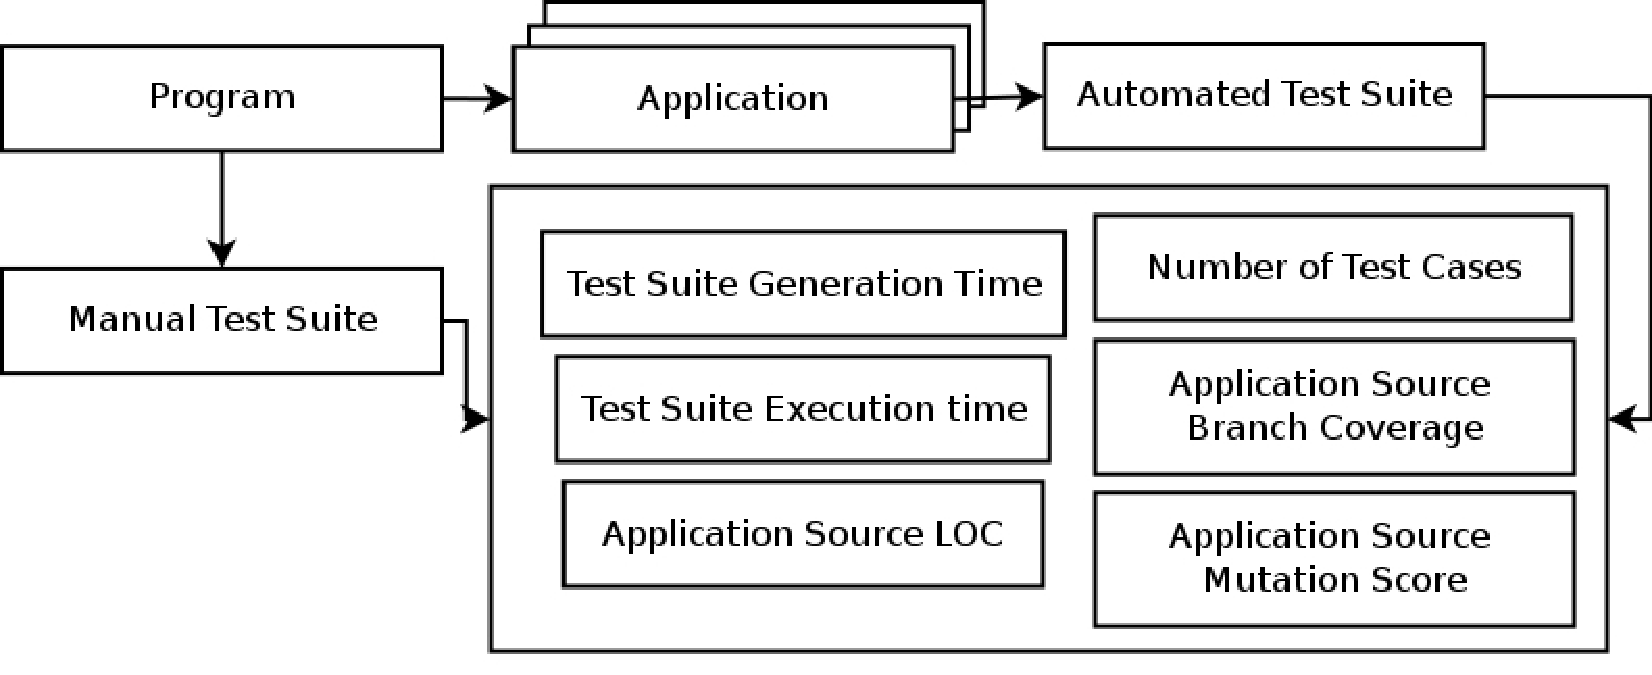
\includegraphics[width=\linewidth]{proccess_diagram.pdf}
    \caption{Evaluation Process}
  \label{fig:process_diagram}
\end{figure}
%KJ: MAKE NEW DIAGRAM!!

\section{Empirical Evaluation}
\label{sec:evaluation}
Given the many different techniques for generating test suites, the primary goal of this paper's empirical study is to compare the quality and complexity of the resulting test suites.  We implemented the empirical evaluation approach as shown in Figure~\ref{fig:process_diagram}.  As can be seen in the figure, existing programs are fed into automatic test suite generators to create executable test suites.  These test suites are then compared to the programs' associated, manually written test suites based on \textcolor{red}{SOME NUMBER} metrics.   

The goals of the experiments are as follows:
\squishlist
\item stuff1
\item stuff2
\item stuff3
\item stuff 4
\squishend

\subsection{Experiment Design and Metrics}
All experiments were performed on GNU/Linux workstations with kernel 3.2.0-44, a 2 GHz Intel Corporation Xeon E5/Core i7 processor and  15.6 GB of main memory. 

\noindent \textbf{Case Study Applications:}  

Ten programs were identified from the SF110 code suite~\cite{fraser:2012}.  The case study applications were selected due to their size, the existence of associated manually developed JUnit test cases, and their use in tuning EvoSuite parameters for mutation and test generation, one of our test suite generation tools.  Table~\ref{tbl:program_table} provides a list of the selected SF110 programs with their respective lines of code (LOC) and average cyclomatic complexity per method.  LOC and cyclomatic complexity were measured using JavaNCSS~\cite{leejavancss}.  

Netweaver is the largest program under consideration with nearly 18K lines of code.  Netweaver has an average Cyclomatic Complexity ($CC$) of 2.82 across all methods, which implies that for a specific method $M$, 1) $CC_M$ is an upper bound for the number of test cases that are necessary to achieve a complete branch coverage within the method $M$, and 2) $CC_M$ is a lower bound for the number of paths through the control flow graph. Assuming each test case takes one path, the number of cases needed to achieve path coverage is equal to the number of paths that can actually be taken, ignoring infeasible paths.  The smallest program, Jni-inchi has around 800 lines of code with an average cyclomatic complexity of 2.05.  

\begin{table}[!t]
\caption{Benchmark Programs and their Properties}
\label{tbl:program_table}
\resizebox{\columnwidth}{!}{%
\begin{tabular}{|l|c|c|}
\hline
\textbf{Program} & \textbf{LOC} &\textbf{Cyclomatic Complexity} \\ \hline
Netweaver                              & 17953                              & 2.82                                                \\ \hline
Inspirento                             & 1769                               & 1.76                                                \\ \hline
Jsecurity                              & 9470                               & 2.05                                                \\ \hline
Saxpath                                & 1441                               & 2.10                                                \\ \hline
Jni-inchi                              & 783                                & 2.05                                                \\ \hline
Xisemele                               & 1399                               & 1.29                                                \\ \hline
Diebierse                              & 1539                               & 1.74                                                \\ \hline
Lagoon                                 & 6060                               & 3.52                                                \\ \hline
Lavalamp                               & 1039                               & 1.50                                                \\ \hline
Jnfe                                   & 1294                               & 1.38                                                \\ \hline
\end{tabular}
}
\end{table}

After the case study applications were identified and analyzed, automated test tools EvoSuite and Codepro were used to generate test suites~\cite{CodePro1, fraser:2011:eat:2025113.2025179}. As EvoSuite is non-deterministic and learning-based, ten sets of tests were generated for evaluation, and the standard deviation is given across the ten test generations for all EvoSuite related results.  

\noindent \textbf{Evaluation Metrics:}

The manually written test suites and automatically generated test suites are compared based upon the time to generate test suites, the number of test cases generated, the time to execute generated tests, lines of code in the benchmark application, complexity of the benchmark application, branch coverage of generated suites, and the mutation score of generated suites. To perform these evaluations, three tools are used.

All tests are written or generated in JUnit form.  The time to generate test cases, number of test cases generated, and the time to execute the test suite are measured using the JUnit tool.  We also measure the non-commented LOC from the source code of the benchmark applications through JavaNCSS~\cite{leejavancss}.  

Following the automatic generation of test cases, Jacoco~\cite{jacoco} is used to calculate branch coverage of the tests.  Jacoco calculates branch coverage by instrumenting all branches at the byte code level through ASM, an all purpose Java bytecode manipulation and analysis framework. We also use MAJOR~\cite{just2011} to calculate fault-based mutation scores given the case study and associated tests. MAJOR is a Java compiler-integrated mutator that serves as a mutation analysis back-end for JUnit tests.  It provides a domain specific language to configure the mutation process, although we used its default values for our experiments.

\subsection{Experiments and Results}
Experiments were run to compare how test suites are generated using automated tools, the differences between the resulting test suites in terms of size and complexity, and the over all quality of the generated test suites.  

\subsubsection{Generating Test Suites }
%Time to generate
\begin{figure*}[!t]
\centering
  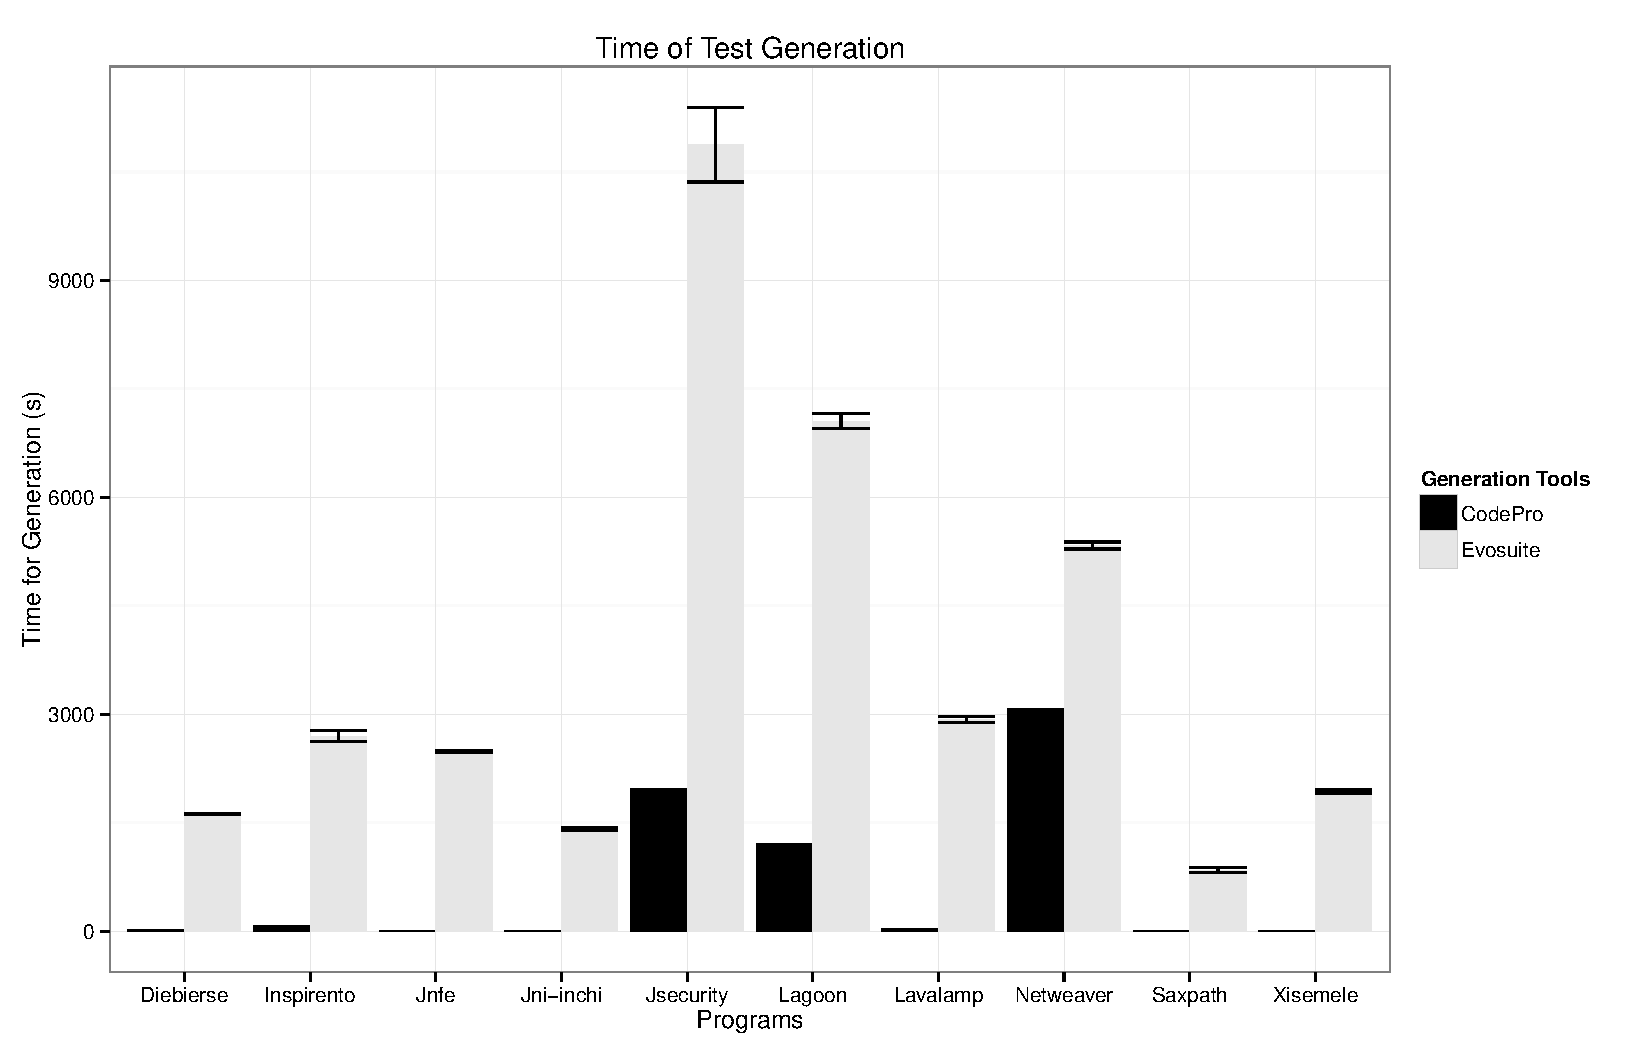
\includegraphics[width=\linewidth]{RGraphs/TimeOfGeneration.pdf}
    \caption{Time to Generate Test Suites.}
  \label{fig:TimeGen}
\end{figure*}
In the first set of experiments, we tracked the time required to generate the test suites, the number of test cases generated, and the execution time of the resulting test suite.  Figure~\ref{fig:TimeGen} displays the time required to generate each test suite using the two automatic test case generation tools, CodePro and \textsc{EvoSuite}.  In the case of Netweaver, CodePro completed test suite generation in approximately 51 minutes whereas \textsc{EvoSuite} required 89 minutes.  This was a small difference of 1.7\% compared to Xisemele, for which CodePro generated a test suite in just 13 seconds compared to 32 minutes from \textsc{EvoSuite}.  The time needed by \textsc{EvoSuite} was 148\% greater in this case.  On average, \textsc{EvoSuite} took 78\% more time in test generation compared to CodePro.

%# of tests
Next, the number of test cases generated per method was analyzed.  Figure~\ref{fig:NumTests} shows the number of tests generated.  For the ten case study applications, CodePro produced an average of  5\% more test cases than \textsc{EvoSuite} and \textcolor{red}{SOME NUMBER} \% more than were written manually.  \textsc{EvoSuite} produced, on average, \textcolor{red}{SOME NUMBER} \% than were created manually. 
\begin{figure*}[!t]
\centering
  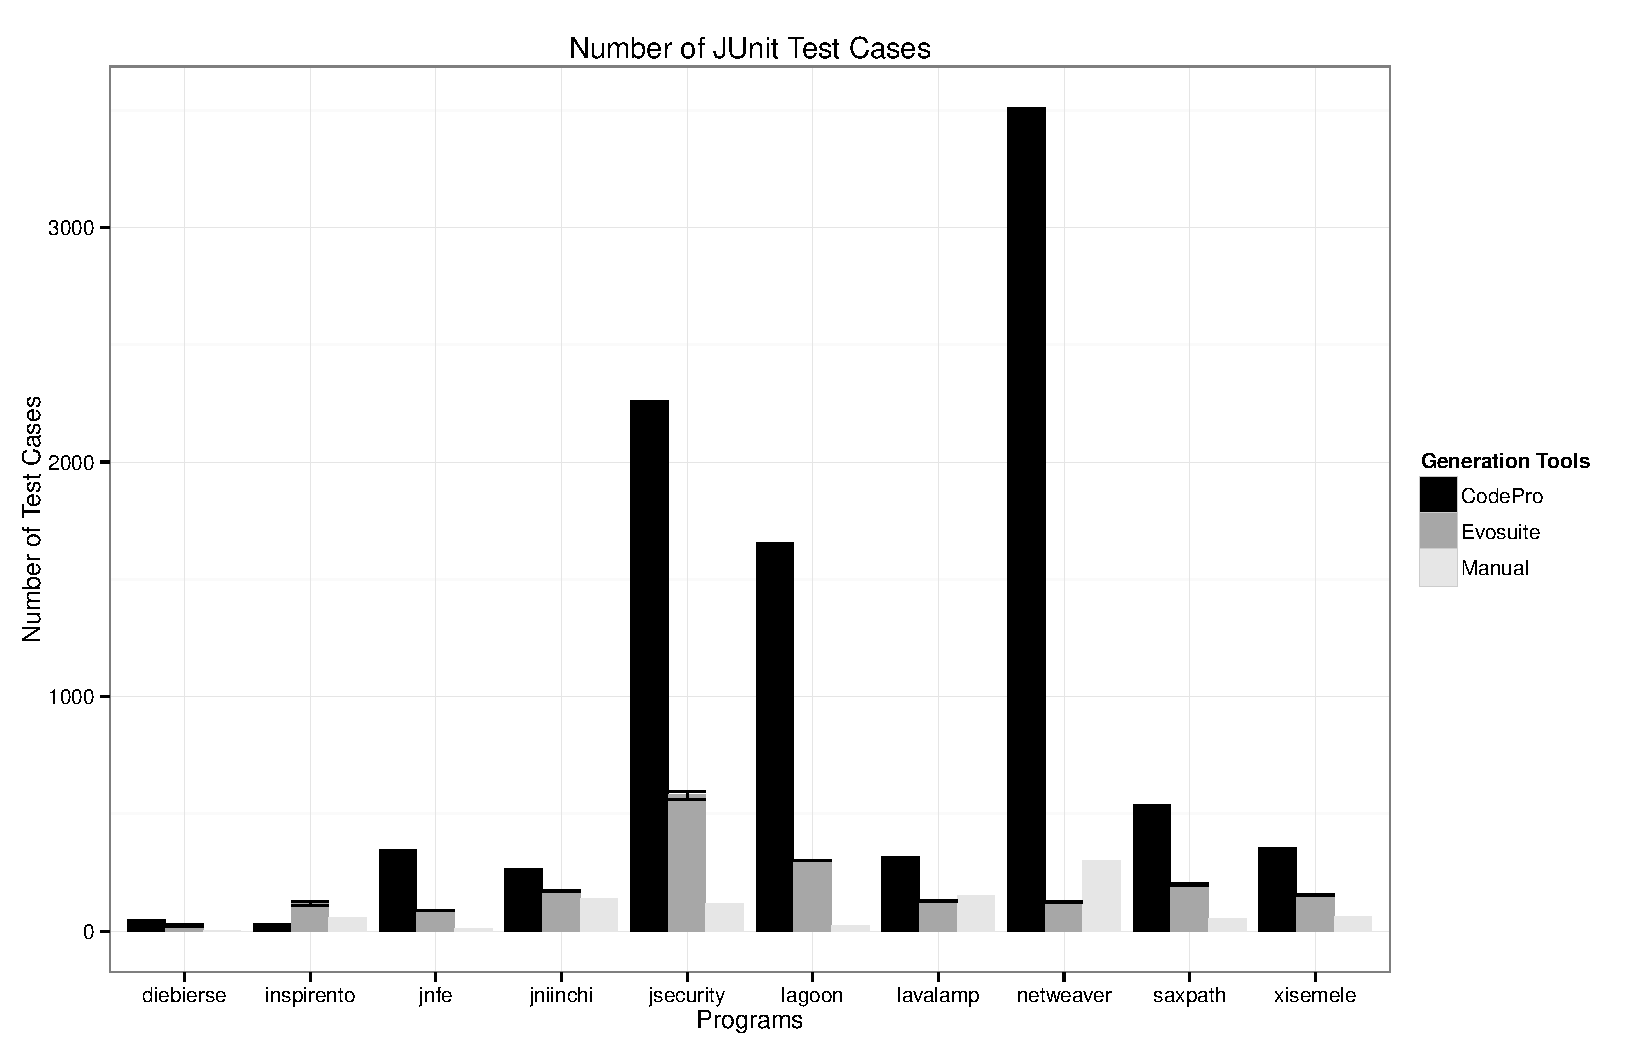
\includegraphics[width=\linewidth]{RGraphs/TestCasesGenerated.pdf}
    \caption{Number of Test Cases per Test Suite.}
  \label{fig:NumTests}
\end{figure*}
%Time of Execution

\subsubsection{Comparing Generated Tests to Case Studies}
%LOC (source)
\begin{figure*}[!t]
\centering
  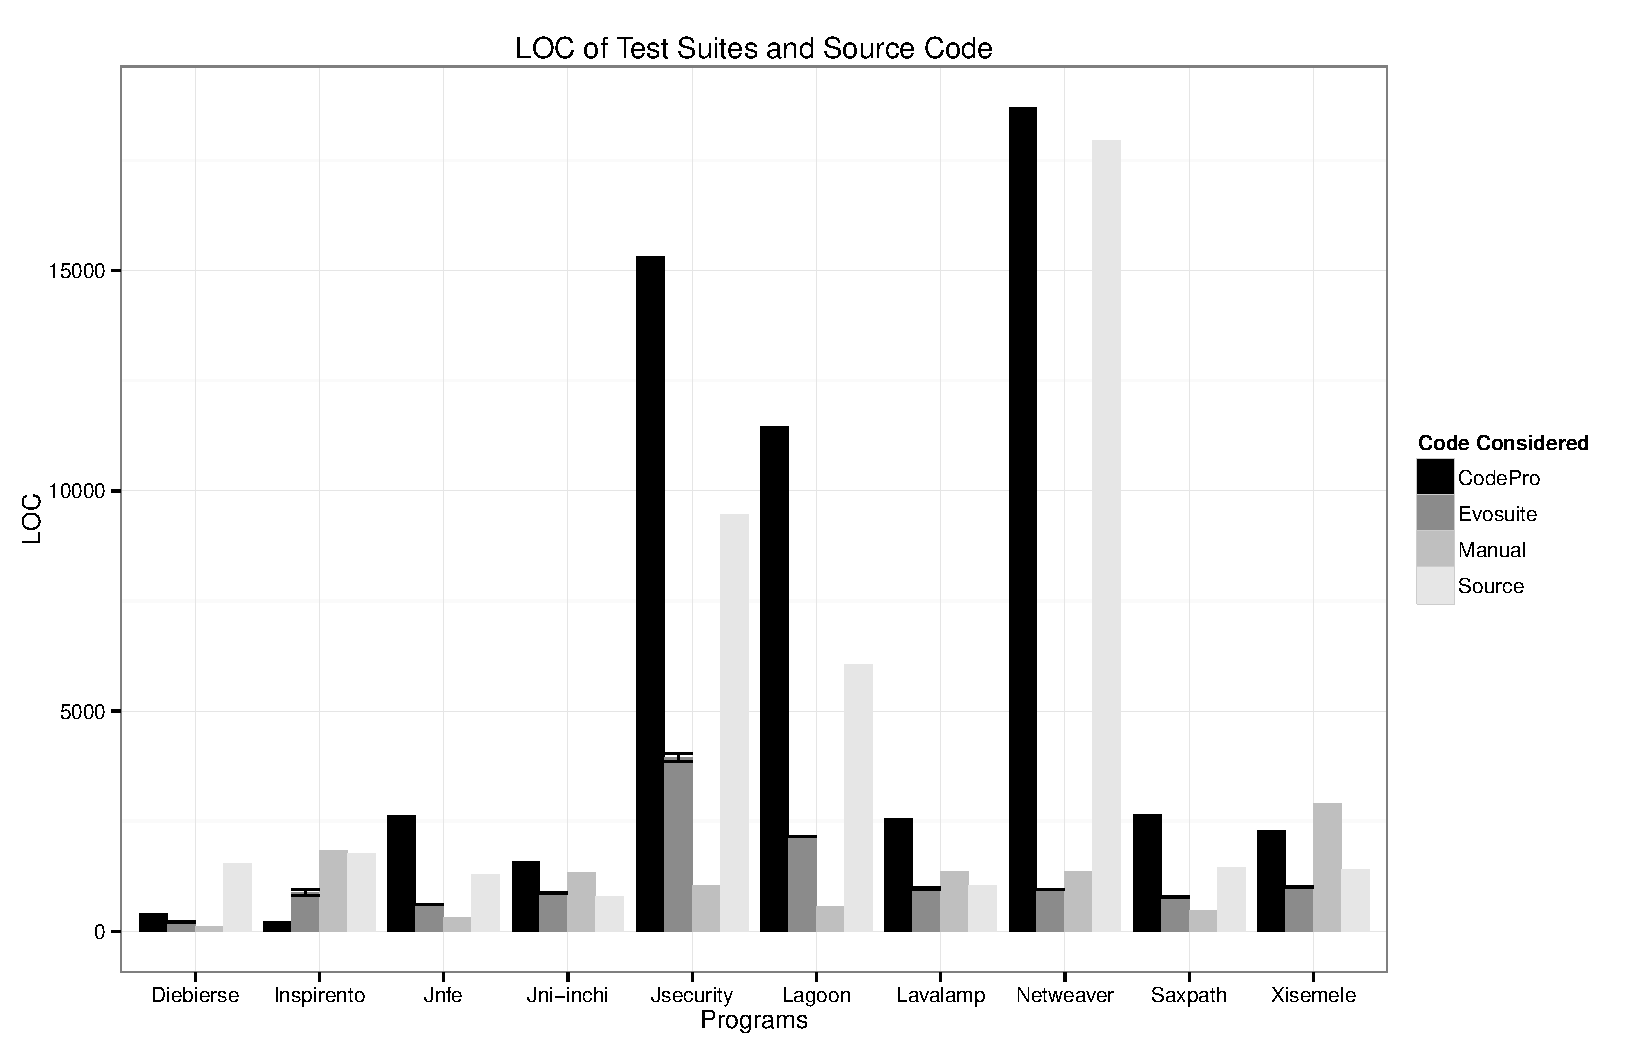
\includegraphics[width=\linewidth]{RGraphs/LOC.pdf}
    \caption{Non-commented lines of code for automatically generated tests and manual tests compared to case study source code. }
  \label{fig:LOC}
\end{figure*}
%Complexity (source)-- do we really compare about complexity of tests versus complexity of source? Leaving out.

\subsubsection{Quality: Manual versus Generated}

%Branch Cov
%Mutation Score
\begin{figure}[!t]
\centering
  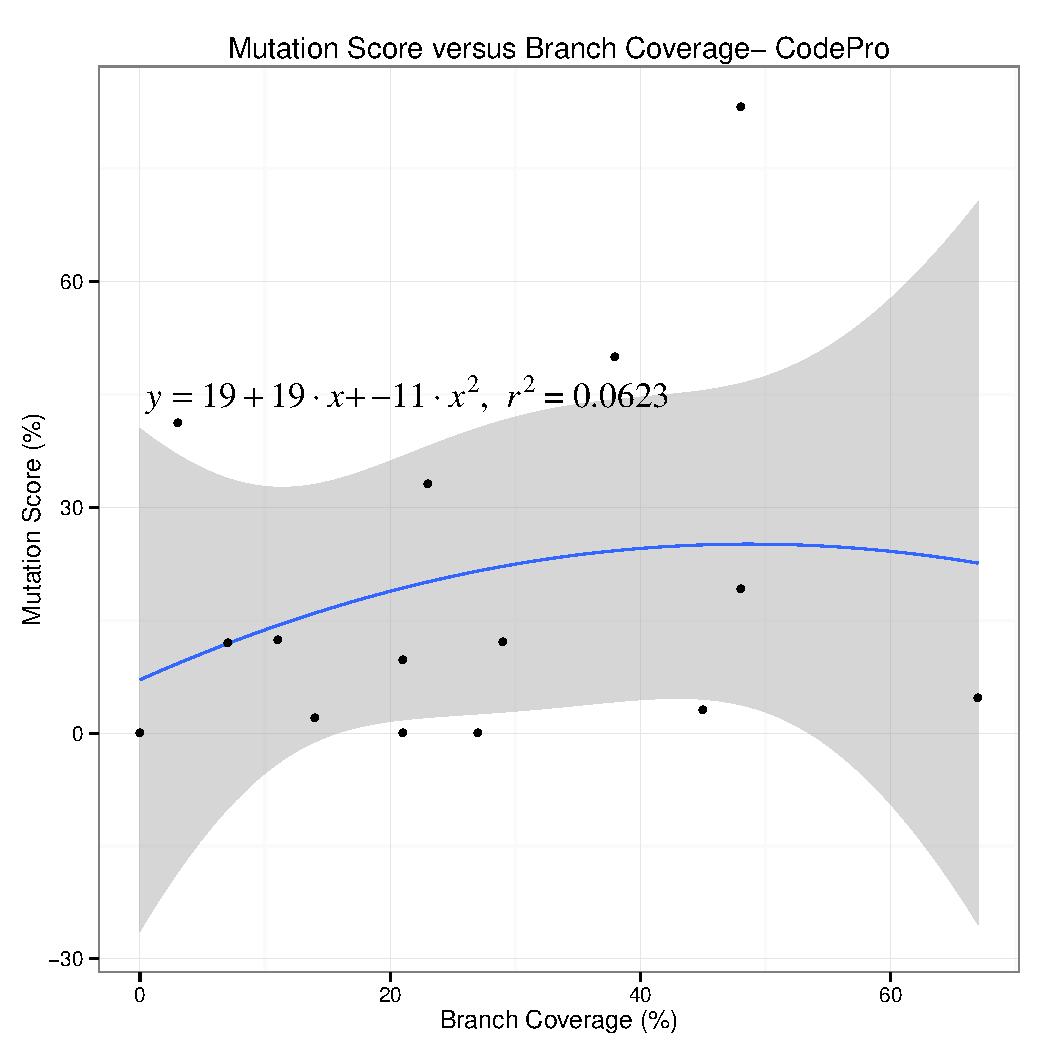
\includegraphics[width=\linewidth]{RGraphs/CodePro_BranchCov_versus_Mutation_poly.pdf}
    \caption{Mutation Score compared to Branch Coverage for test suites generated by CodePro.}
  \label{fig:CP_branch_mutation}
\end{figure}
\begin{figure}[!t]
\centering
  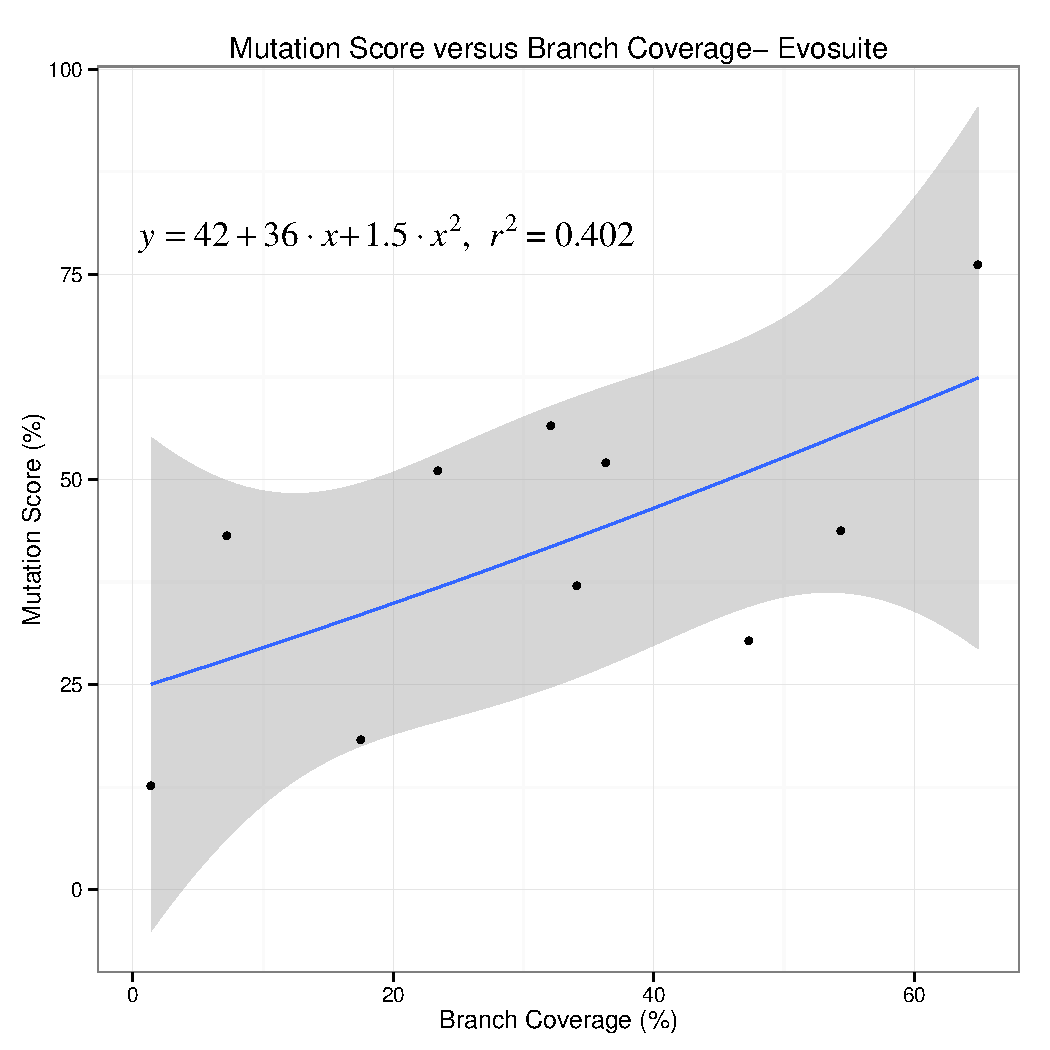
\includegraphics[width=\linewidth]{RGraphs/Evosuite_BranchCov_versus_Mutation_poly.pdf}
    \caption{Mutation Score compared to Branch Coverage for test suites generated by Evosuite.}
  \label{fig:Evo_branch_mutation}
\end{figure}
\begin{figure}[!t]
\centering
  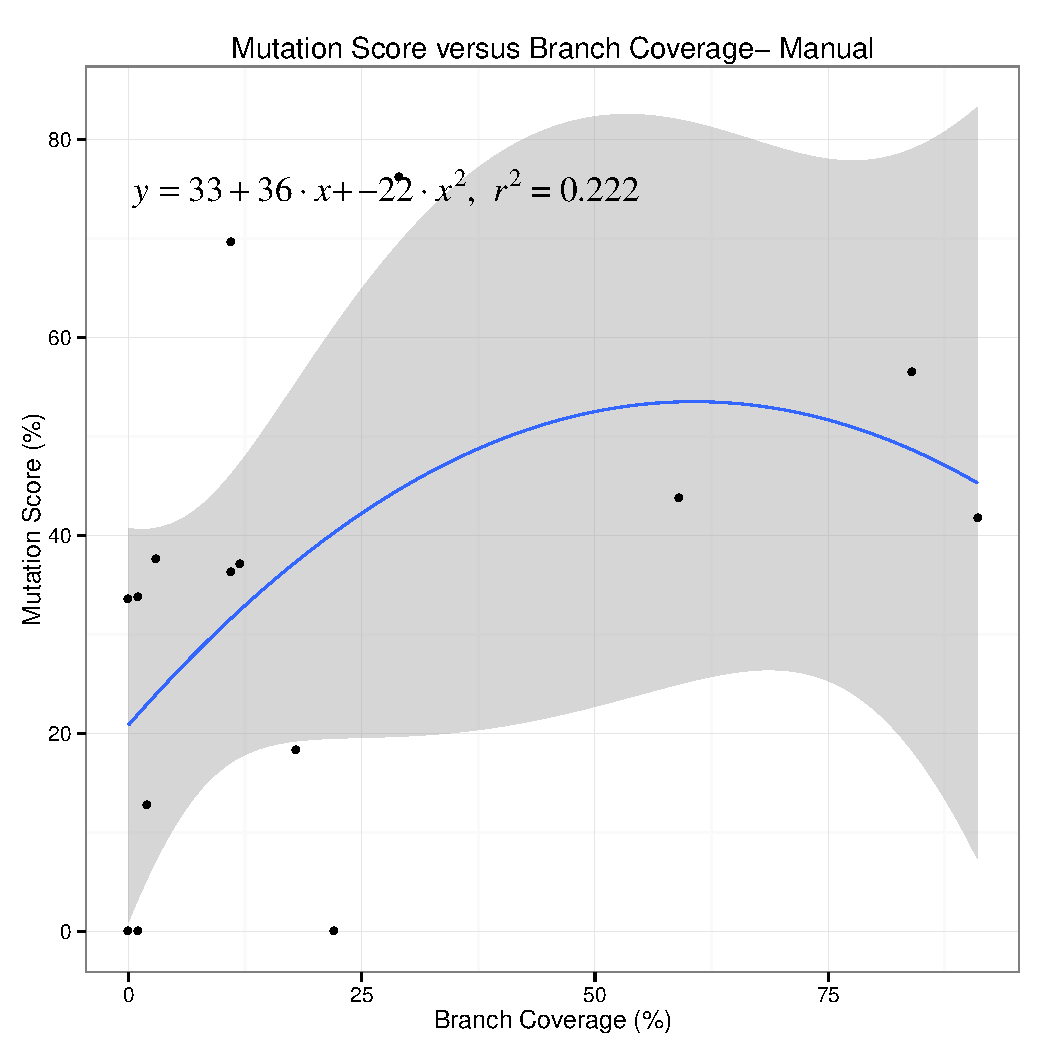
\includegraphics[width=\linewidth]{RGraphs/Manual_BranchCov_versus_Mutation_poly.pdf}
    \caption{Mutation Score compared to Branch Coverage for test suites created manually.}
  \label{fig:manual_branch_mutation}
\end{figure}


\subsection{Threats to Validity}
\noindent \textbf{Internal Validity}
Threats to internal validity include the 

Measurements in quality of software tests is a subjective measurement. Although mutation score is one way to measure the quality of a test suite, ignoring the human elements of tests are nigh impossible. Developers may need to view tests in order to diagnose faults in the code, and if a developer cannot understand the test they are reading, then the cost of time and effort could be increased on the human part.

The statistical analysis also may be a threat to validity, as the inconsistency in how both Evosuite and manually written tests are created. Also, CodePro generated some test suites with a mutation score of 0, which could mislead one to believing that CodePro has no use for creating quality tests. For this reason we removed these results to give a better impression of the trend CodePro test suites.

\noindent \textbf{External Validity}

\noindent \textbf{Construct Validity}
